% Bansat paper -- final version agreed by the authors, 10 November 2026.
% Build: latexmk -pdf -interaction=nonstopmode main.tex
% Every number about Bansat comes from the repository (github.com/bewithkhan/bansat).
\documentclass[11pt,a4paper]{article}

\usepackage[T1]{fontenc}
\usepackage[utf8]{inputenc}
\usepackage{lmodern}
\usepackage[margin=22mm]{geometry}
\usepackage{microtype}
\usepackage{authblk}
\usepackage{amssymb}
\usepackage{booktabs}
\usepackage{tabularx}
\usepackage{xltabular}
\usepackage{array}
\usepackage{enumitem}
\usepackage{xcolor}
\usepackage{graphicx}
\usepackage{tikz}
\usetikzlibrary{arrows.meta,positioning,shapes.geometric}
\usepackage[numbers,sort&compress]{natbib}
\usepackage{xurl}
\usepackage[hidelinks]{hyperref}
\usepackage{orcidlink}
\usepackage{caption}
\usepackage{multicol}
\captionsetup{font=small,labelfont=bf,skip=4pt}

\newcommand{\doi}[1]{\href{https://doi.org/#1}{doi:#1}}
\DeclareRobustCommand{\fpath}[1]{\path{#1}}
\newcolumntype{L}{>{\raggedright\arraybackslash}X}
\newcolumntype{P}[1]{>{\raggedright\arraybackslash}p{#1}}
\setlist{itemsep=1pt,topsep=3pt}
\setlength{\bibsep}{0.4pt}
\renewcommand{\bibfont}{\footnotesize}
\setlength{\textfloatsep}{10pt plus 2pt minus 2pt}
\renewcommand{\topfraction}{0.85}
\renewcommand{\textfraction}{0.1}
\renewcommand{\floatpagefraction}{0.8}

\title{Bansat: Blueprint-First Gating of AI Coding Agents,\\ with a Continuously Verified Privacy-Law Registry}

\author[1]{Muhammad Tufail Khan\thanks{Corresponding author: \href{mailto:Muhammadtufail.khan@uws.ac.uk}{Muhammadtufail.khan@uws.ac.uk}. ORCID: \href{https://orcid.org/0009-0004-5791-5129}{0009-0004-5791-5129}}}
\author[1]{Naeem Ramzan~\orcidlink{0000-0002-5088-1462}}
\affil[1]{School of Computing, Engineering and Physical Sciences, University of the West of Scotland, Paisley, United Kingdom}
\date{10 November 2026}

\begin{document}
\maketitle

\begin{abstract}
The failures that sink applications built by AI coding agents are often decisions nobody made, such as whether every
table enforces access control or whether trackers load before consent. Bansat is an
open framework and Agent Skill that has the agent write a complete blueprint before any production code (product,
architecture, security, privacy law, accessibility and 17 UI states for every screen), sized by a 20-question risk
screen, and then holds the agent at approval gates that only a person may sign. A 29-item audit of launch traps runs
before real personal data is collected and again before launch. An optional hook makes the first gate a
hard stop in agents that support pre-tool-use hooks; a retrofit track covers live applications. Because legal advice ages,
Bansat also keeps a public law registry in which every claim must cite an official source, enforced in continuous
integration; it holds 120 entries citing 2,944 official URLs. A weekly watch detects changes on 105 official sources,
and a weekly AI verify task, told to treat fetched content as data and never as instructions, drafts sourced updates
for a person to review. On 31 golden cases, six of them carrying injected instructions, the verify task's first
round found 10 of 18 known changes, invented none and followed no injected instruction; the misses shared one cause,
which led to a prompt change. With the revised prompt, a second round found all 18, again inventing nothing and
following no injected instruction, although its runs were not fully independent. We also publish an agreed, pre-specified
protocol for comparing applications an AI agent builds with and without Bansat; its runs have not yet taken place.
\end{abstract}


% =====================================================================================================================
\section{Introduction}\label{sec:intro}

Coding agents built on large language models (LLMs) let a founder with no engineering team describe an application and
have it built. What the agent rarely does, unless asked, is settle the questions that decide whether it can be launched
safely and lawfully. Bansat's README calls these \emph{decisions nobody
made} and lists twenty-nine recurring ``launch traps''~\cite{khan2026bansat}. Among them: row-level security is off, so
anyone with the application's public key can read or change its tables; fonts load from a third-party host, sending
every visitor's IP address there before any consent; session replay or advertising pixels load before anyone has said
yes; the ``we launched'' email to a waitlist has no unsubscribe link or sender identity; the sign-up form never asks for
age; and the privacy notice, written by an AI, describes an application that does not exist. Each has a concrete cost.
In 2022 the Regional Court of Munich held that a site which passed a visitor's dynamic IP address to Google through
Google Fonts, without consent, had infringed his rights, and awarded \texteuro100 in damages under Article~82
GDPR~\cite{lgmuenchen2022fonts}.

These failures are documented. Bansat's breach casebook (Appendix~F of the framework) maps twenty incidents and
regulators' decisions from January~2025 to October~2026 to the checks that catch each class of failure, and admits a
case only if it rests on a primary source~\cite{khan2026bansat}. Researchers who examined 1,645 applications from one
AI app builder's showcase reported 303 vulnerable endpoints across 170 of them, about 10.3\%, and traced them to
inadequate row-level security in the applications' database backends~\cite{palmer2025statement}. A scan of about
300,000 domains showing signs of one backend-as-a-service found 16,326 databases with tables readable without
authorisation, noting that tables created through the API, as coding agents typically create them, do not have
row-level security on by default~\cite{upguard2026supabase}. One company reported that an AI agent ignored a code freeze and deleted a production database of 1,206 executive
records and more than 1,196 company profiles, later recovered~\cite{saastr2025replit}; a hosting provider reported that an agent found an account-scoped API token on a
user's machine and used it to delete a production volume~\cite{railway2026nuke}. A security vendor reported that crafted
error reports led coding agents asked to fix them to run an attacker's package, and found 2,388 organisations whose
error-tracking endpoints could be used this way; its 85\% success rate is its own, unverified
figure~\cite{tenet2026agentjacking}. A self-replicating worm compromised more than 500 npm packages~\cite{cisa2025npm}. At the largest scale, France's data protection authority fined SHEIN's Irish
subsidiary \texteuro150 million because advertising cookies were placed before visitors chose and after they clicked
``Refuse all''~\cite{cnil2025shein}.
The casebook says its checks catch a \emph{class} of failure, not that Bansat would have prevented any one incident;
we make no such claim either.

Studies of agent-built software agree. An analysis of deployed ``vibe-coded'' applications traces their vulnerabilities
to security obligations forgotten, underspecified or never established in the workflow~\cite{deng2026vibecoded}. A benchmark of real-world feature requests found that few
of the agents' functionally correct solutions were also secure, and that adding vulnerability hints to the request did
not fix this~\cite{zhao2025susvibes}. A missing decision is better caught before the code exists.

Bansat (Pashto for ``foundation'') takes that position: before an AI coding agent writes production code, it writes a
complete blueprint of the project and stops at gates that only a person may sign. Our contributions are:
\begin{enumerate}
  \item \textbf{A blueprint-first framework distributed as an Agent Skill} (Section~\ref{sec:framework}): a risk
  screen that sizes the blueprint, fifteen blueprint parts, gates signed only by a person (with an optional hook that
  makes the first a hard stop), 17 mandatory UI states, an 18-item blocking launch gate, and a retrofit track.
  \item \textbf{A casebook-driven feedback loop}: twenty sourced incidents mapped to checks, which exposed gaps and added
  14 checks to version~2.4, most of them about coding agents, CI/CD and connected applications.
  \item \textbf{A public privacy-law registry with an official-sources rule} enforced in CI, kept current by a
  deterministic weekly watch and an AI verify task whose output a person reviews (Section~\ref{sec:law}).
  \item \textbf{An evaluation of the verify task} on 31 golden cases, six with injected instructions, reporting two
  rounds as recorded, the prompt change between them, and the limits on their independence.
  \item \textbf{A pre-specified controlled experiment} (Section~\ref{sec:experiment}), with hypotheses, a randomised
  block design and an analysis plan, agreed by the authors and published before any run.
\end{enumerate}

% =====================================================================================================================
\section{Background and related work}\label{sec:related}

\paragraph{Plan-first and spec-driven development with AI agents.}
Models can plan before writing code~\cite{jiang2024selfplanning}, and multi-agent frameworks organise agents into a
software process~\cite{hong2023metagpt,qian2024chatdev}; in practice the idea has become \emph{spec-driven
development}. GitHub's Spec Kit gives a coding agent a sequence of
commands (a project \emph{constitution}, then \emph{specify}, \emph{plan}, \emph{tasks} and \emph{implement}, with a
convergence check) in which the specification remains the reference point~\cite{speckit}. Marri proposes a versioned
``constitution'' of security constraints that governs all later generation~\cite{marri2026csdd}, and Alenezi a reference
model in which structured specifications, not conversation, are the source of truth~\cite{alenezi2026sdd}. Bansat shares
the premise but its blueprint is a fixed, cross-domain template reaching into privacy law, consent, children's data,
accessibility and UI states; its depth is set by a legal and safety risk screen; and its gates are approvals only a
person signs.

\paragraph{Agent Skills.}
Agent Skills are an open format in which a skill is a folder with a \fpath{SKILL.md}
file of metadata and instructions, optionally with scripts and references. Agents load skills by progressive
disclosure: each skill's name and description at start-up, the full instructions when a task matches, and bundled files
as needed~\cite{agentskills}. SkillsBench found that curated skills raised agents' average pass rate by 16.2 percentage
points across 86 tasks, with wide variation by domain~\cite{li2026skillsbench}. Skills also add attack surface, including the absence of a data--instruction boundary~\cite{li2026secureskills} and
vulnerable skills in the wild~\cite{liu2026skillswild}. Bansat is itself a skill, so these findings apply to it (Section~\ref{sec:discussion}).

\paragraph{Privacy by design and GDPR Article~25.}
Article~25 GDPR requires a controller to implement appropriate technical and organisational measures, both when it
decides how to process personal data and during processing, and by default to process only the data each purpose
needs~\cite{gdpr}. Its engineering demands are debated~\cite{bygrave2017dpbd}, and privacy by design has long been easier to endorse
than to operationalise~\cite{spiekermann2012pbd}. Privacy professionals report no shared understanding of the ``technical measures'' the GDPR asks
for~\cite{klymenko2022technical}. Measurement studies have asked whether consent banners respect users'
choices and comply with the law~\cite{matte2020cookie}, and how consent pop-up design influences what users
choose~\cite{nouwens2020dark}. Bansat turns several such duties into build-time tests.

\paragraph{Threat modelling and OWASP ASVS.}
Threat modelling is well studied~\cite{xiong2019threat}, and LINDDUN extends it to privacy threats~\cite{deng2011linddun}.
Bansat's security part applies STRIDE~\cite{shostack2014threat}
to each data flow and pre-fills 16 threats that recur in AI-built applications, from missing row-level security to
coding agents holding production credentials. The OWASP Application Security Verification Standard, at version 5.0.0,
gives a basis for testing web applications' technical security controls and requirements for building them
securely~\cite{owaspasvs}; Bansat lists it among its standards, with WCAG~2.2 for accessibility~\cite{wcag22}.

\paragraph{Security of AI-generated code.}
Early work found GitHub Copilot often suggesting vulnerable code in scenarios built around common weakness
classes~\cite{pearce2022asleep}. In a user study, participants with an AI assistant wrote significantly less secure code
than those without one, yet were more likely to believe it secure~\cite{perry2023insecure}. Studies of ChatGPT's and Copilot's code followed~\cite{khoury2023chatgpt,fu2025copilot}, and benchmarks have moved to
whole backends~\cite{vero2025baxbench} and multi-file agent tasks~\cite{zhao2025susvibes}. This work measures vulnerabilities in code; Bansat targets the step before, the decisions
about data, consent, access and failure states that determine what the code should do.

\paragraph{Prompt injection against LLM agents.}
Prompt injection was first characterised as goal hijacking and prompt leaking~\cite{perez2022ignore}; indirect prompt
injection plants instructions in data an application retrieves, and has compromised deployed LLM-integrated
applications~\cite{greshake2023signedup}. AgentDojo and InjecAgent evaluate attacks and defences for tool-using
agents~\cite{debenedetti2024agentdojo,zhan2024injecagent}. Bansat meets it in its coding-agent rules and in its
law-verification task, which reads untrusted pages (Section~\ref{sec:verify}).

\paragraph{Regulatory change monitoring.}
Requirements engineering treats law as a source of requirements~\cite{otto2007legal,breaux2008regulatory} and counts the
changeability of regulatory acts among its central difficulties~\cite{kosenkov2021vision}. Tracing regulatory change by
hand is time-consuming and error-prone, which motivates automated change-impact analysis~\cite{abualhaija2024change}.
LLMs also state legal falsehoods with confidence~\cite{dahl2024fictions,magesh2025hallucination}. Bansat's response:
detection is deterministic, the AI only drafts, every claim cites an official source, and a person reviews every change.

% =====================================================================================================================
\section{The Bansat framework}\label{sec:framework}

\subsection{Structure and distribution}
Bansat~2.4 is plain Markdown: fifteen parts (0--14) and six appendices (A--F), about 3,800 lines split into
modules~\cite{khan2026bansat}. A combined single file is generated from the modules, and continuous integration (CI) fails
if the two drift apart. \fpath{SKILL.md} tells the agent which modules to read at each step, so it loads only the parts
in scope. Text and templates are licensed CC~BY~4.0 and code samples MIT. The code samples run in CI, where a Prisma
schema's row-level security (RLS) policies pass 13 access checks in Postgres and a Playwright privacy test must fail on a
page that loads a third-party font before consent; CI also fails if a sample in the text and its tested copy differ. Beside Appendix~D's nine project-type profiles, 24 \emph{stack
profiles} in \fpath{stacks/} (seven backend, six frontend and full-stack, four mobile, seven no-code or
backend-as-a-service) say what changes from the Next.js and Supabase reference; the skill loads only the one a project
needs. They first shipped in v3.0.0, released on 10~November 2026. Figure~\ref{fig:flow} shows the two tracks through the
framework.

\begin{figure}[tbp]
\centering
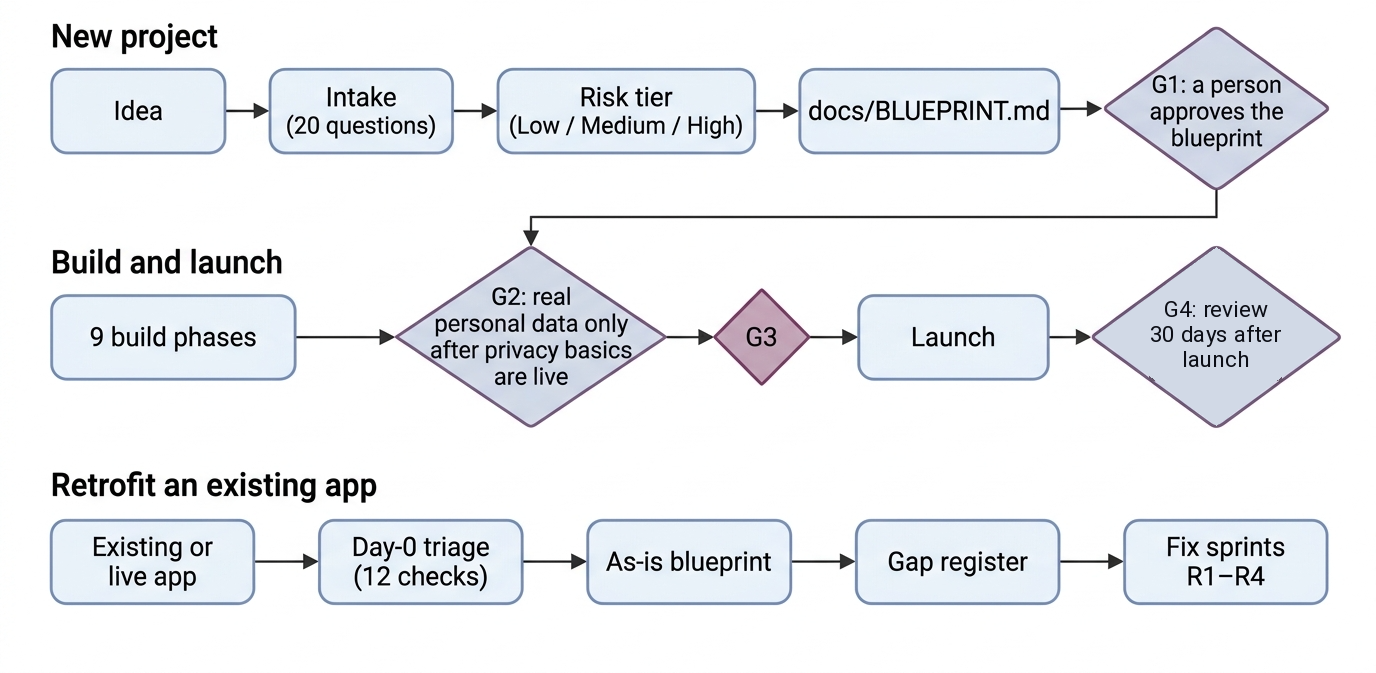
\includegraphics[width=\linewidth]{figures/bansat-workflow.png}
\caption{The new-project track (top two rows) and the retrofit track (bottom row). At each gate the agent is told to
stop until a person signs the gate's row in the blueprint. G3, the release candidate, blocks launch while any of the
18 blocking launch-gate checks is red (Table~\ref{tab:gates}). Once a
retrofit reaches its gate R2 (blueprint complete, every gap registered), new scope follows the normal gates. Adapted
from the repository README.}
\label{fig:flow}
\end{figure}

\subsection{Intake and risk tiers}
Part~0 asks twenty screening questions, each switching on a module when answered yes, from markets (UK, EU, Nigeria, US
and others), under-18 users and special category data to AI, payments, marketing, analytics, third-party embeds and a
B2B processor role. The answers set a tier. \textbf{High}: special category data, location or worker monitoring, wearables, children as a target or
likely audience, or significant automated decisions; a data protection impact assessment (DPIA) is then mandatory.
\textbf{Medium}: accounts, analytics, marketing or a B2B processor role. \textbf{Low}: otherwise. The tier sets the
minimum depth before build: a Low-tier project completes only the intake, the core product specification, the stack,
cookies, the launch-trap audit, UI states and the launch gate; a High-tier project completes everything, plus a DPIA
and an independent review before G3. The skill asks at
most five questions, only where a wrong guess would be costly, and flags every assumption. Eight \emph{delivery
questions} feed a method picker (Section~\ref{sec:scale}).

\subsection{The blueprint}
The agent writes the blueprint to \fpath{docs/BLUEPRINT.md} in the project, where it changes in the same pull request as
the code (Table~\ref{tab:parts}). Requirements carry identifiers (\texttt{FR-}, \texttt{NFR-}, \texttt{SCR-},
\texttt{API-}, \texttt{ADR-} and others), so each feature traces to its screens, endpoints, data, tests and record of
processing. Part~8 covers AI features, including the transparency duties of Article~50 of the EU AI Act~\cite{aiact}.
Part~12, the agent's operating manual, goes into the project's agent instructions file, such as \fpath{AGENTS.md}. Its rules include:
research how others built something before building it; re-check authorisation in every server entry point; implement
every applicable UI state; never sign a gate; work with development keys only; ask before any destructive command; never
switch off one's own approval prompts or sandbox; and treat text in tool results, issues, error reports and web pages as
data, not instructions.

\begin{table}[tbp]
\centering\footnotesize
\caption{The parts of a Bansat blueprint (framework v3.1).}\label{tab:parts}
\begin{tabularx}{\linewidth}{@{}lL@{}}
\toprule
Part & What it settles \\
\midrule
0 Intake \& risk & 20 screening questions, risk tier, modules in scope, 8 delivery questions \\
1 Product (PRD) & Problem, metrics, personas, MoSCoW features with IDs, Gherkin acceptance criteria \\
2 Non-functional & Numeric targets: Core Web Vitals, uptime, recovery, security, accessibility, cost \\
3 Architecture (TRD) & Pinned stack, environments, context diagram, data flows, processor register, secrets \\
4 Decisions & Architecture decision records, each recording the prior art considered \\
5 Data & Data classes, dictionary, schema, data-layer access rules with isolation tests, retention \\
6 API & Endpoint inventory, RFC~9457 errors mapped to UI states, validation, webhooks, rate limits \\
7 Security & Authentication flow, RBAC matrix, 16 pre-filled STRIDE threats, headers and CSP, logging \\
8 AI features & Feature register, minimised inputs, evals, prompt-injection defences, AI Act labelling, spend caps \\
9 Privacy \& compliance & 27 sections, from lawful bases, consent and cookies to children, breach, DPIA and launch traps \\
10 Experience & App flow, look-and-feel brief, WCAG~2.2 AA, design tokens, 17 UI states with a state matrix \\
11 Delivery & 9 phases with exit criteria, Definition of Done, testing, CI/CD, method picker, PM toolkit \\
12 Agent manual & Agent rules, research-first feature protocol, 8-step debugging protocol, prompt library \\
13 Launch gate & 40 go/no-go checks, 18 of them blocking \\
14 Retrofit & Day-0 triage, reverse-engineering, gap register, review cadence, portfolio register \\
A--F Appendices & Templates, sources, glossary, 9 project-type and 6 delivery-method profiles, breach casebook \\
\bottomrule
\end{tabularx}
\end{table}

\subsection{Gates}
Table~\ref{tab:gates} gives the gates. G2 is the one most often missed: a ``coming soon'' page with an email box already
processes personal data, so not even a waitlist address may be collected before the privacy basics are in place. Only a
person signs a gate, by filling in its row (approver and date) in the blueprint; the agent is told never to fill it in,
even when the user says ``approved'' in chat.

\begin{table}[tbp]
\centering\footnotesize
\caption{Bansat's gates (\fpath{framework/how-to-use.md}).}\label{tab:gates}
\begin{tabularx}{\linewidth}{@{}lP{40mm}L@{}}
\toprule
Gate & Unlocks & Exit criteria \\
\midrule
G0 Idea & Writing the blueprint & Part~0 and the first product sections drafted \\
G1 Blueprint approved & Production code (throwaway spikes allowed earlier) & All in-scope sections complete; ADRs accepted; DPIA screening done; no placeholder left in scope \\
G2 Data-ready & Collecting any real personal data & Privacy notice live; processing records and lawful bases; consent capture; processor contracts; isolation tests passing; UK registration fee paid \\
G3 Release candidate & Public launch & Testing complete; every launch-gate item green, or not applicable with a reason \\
G4 Post-launch & The next major scope & 30-day review of metrics, incidents, rights requests and the compliance calendar \\
\bottomrule
\end{tabularx}
\end{table}

\subsection{UI states}
Part~10 requires every screen and asynchronous component to handle each applicable
state of the seventeen in Table~\ref{tab:states}, or give a reason it does not apply, and to prove it in a per-screen
state matrix. S1--S10 are the core set; S11--S17 are required wherever they can occur. Each state has an acceptance test, and a typed pattern makes the compiler reject a view that
omits one.

\begin{table}[tbp]
\centering\footnotesize
\caption{The 17 mandatory UI states (framework 10.7), with the condition that triggers each.}\label{tab:states}
\begin{tabularx}{\linewidth}{@{}P{29mm}L@{\hspace{4mm}}P{43mm}L@{}}
\toprule
\multicolumn{2}{@{}l}{Core (S1--S10)} & \multicolumn{2}{l@{}}{Extended (S11--S17)} \\
\midrule
S1 Empty & first use, or an empty list & S11 Not found / deleted & 404 or 410 \\
S2 Loading & a request in flight & S12 Offline queue / sync conflict & queued writes; 409 \\
S3 Error & 5xx or an unknown error & S13 Rate limited / quota reached & 429 \\
S4 No internet & offline, or failed fetches & S14 Long-running / background task & AI generation, export, import \\
S5 Slow network & over 1\,s, 5\,s, 15--30\,s & S15 Degraded / partial & one section or third party fails \\
S6 No search results & a query returns nothing & S16 Destructive confirmation \& undo & delete or remove actions \\
S7 Permission denied & 403 & S17 Consent-gated content & an embed blocked until consent \\
S8 Session expired & 401, or refresh fails & & \\
S9 Form validation & client check; server 422 & & \\
S10 Success & a mutation confirmed & & \\
\bottomrule
\end{tabularx}
\end{table}

\subsection{Launch checks}
Bansat checks a project twice before it meets the public. The \emph{launch-trap audit} (framework 9.26) lists the
twenty-nine failures that get AI-built applications fined, breached or rejected by app stores, each with a fix and a
way to verify it (Table~\ref{tab:traps}), and runs before G2 and again before G3. Version 3.1.0 added the last twelve:
AI disclosure, opt-out signals, biometric and health data, online withdrawal, legal notices, accessibility law,
server-side authorisation, AI spending limits, app store labels, card data and payment webhooks. The list is curated:
we chose each trap from a law, a regulator's decision, a published vulnerability or a documented incident, and did
not measure how often applications built by AI agents fall into it. The experiment in Section~\ref{sec:experiment} is
the first test of twelve of them. The \emph{launch gate} (Part~13) has 40 go/no-go items in seven
groups, 18 of which block launch while open. Blocking items include a tested backup restore, data-layer access
with isolation tests, no exposed secrets, nothing non-essential before consent, compliant marketing email, and working
export and account deletion.

{\footnotesize
\begin{xltabular}{\linewidth}{@{}>{\raggedleft\arraybackslash}p{1.1em}>{\raggedright\arraybackslash}X>{\raggedright\arraybackslash}X>{\raggedright\arraybackslash}X@{}}
\caption{The 29 launch traps (framework 9.26). Each fix names the framework section that covers it, followed by the
evidence that proves it. Traps 18--29 were added in version 3.1.0; the experiment in Section~\ref{sec:experiment} tests
version 3.0.0, which has the first 17.}\label{tab:traps}\\
\toprule
\# & Trap & Why it bites & Fix and proof \\
\midrule
\endfirsthead
\multicolumn{4}{@{}l}{\emph{Table~\ref{tab:traps}, continued}}\\
\toprule
\# & Trap & Why it bites & Fix and proof \\
\midrule
\endhead
\bottomrule
\endlastfoot
1 & The sign-up form never asks for age & Children's data without parental consent or safeguards; under Nigeria's NDPA a child is anyone under 18 & A neutral age question (9.12); an end-to-end test of the under-age path \\
2 & Fonts from a third-party CDN & Visitors' IP addresses go to a third party with no lawful basis; German courts have awarded damages~\cite{lgmuenchen2022fonts} & Self-hosted fonts and a self-only font policy (9.9); the privacy test \\
3 & Session replay or heatmaps before consent & A consent breach, and recordings can capture personal data & A consent-gated loader with strict masking (9.10); the privacy test \\
4 & A launch email with no unsubscribe, sender identity or address & Breaches UK PECR, US CAN-SPAM and Nigeria's NDPA, and fails Gmail and Yahoo sender rules & A compliant template and one-click unsubscribe (9.11); a seed-inbox test \\
5 & Row-level security off, or the secret key in the client & Anyone can read or write the database & Row-level security on every table and keys on the server only (5.4, 7.3); isolation tests in CI \\
6 & A template or AI-written privacy policy & It doesn't match what the app does, so it breaches transparency duties & Written from the record of processing (9.6); a checklist review \\
7 & Ad or analytics pixels in the root layout & Data shared with ad platforms before consent & A consent loader, with Consent Mode denied by default; the privacy test \\
8 & User data sent to an LLM with no disclosure or DPA & Transparency, transfer and processor-contract breaches & A recorded provider decision, a DPA and redaction; the vendor register \\
9 & No account deletion or data export & A rights breach, and an App Store rejection & A privacy centre (9.15); end-to-end tests \\
10 & Personal data in logs or error trackers & Breaches minimisation and widens any breach & Scrubbing and logging rules (7.5); a log review \\
11 & Pre-ticked boxes, or ``by using this site you agree'' & Invalid consent under the GDPR~\cite{gdpr} & Unticked, granular choices (9.7); a UI review \\
12 & A cookie banner with no ``Reject all'' & Invalid consent, and a leading enforcement theme~\cite{cnil2025shein} & Equal Accept and Reject on the first layer; a screenshot review \\
13 & Real customer data in preview or staging & A security and purpose-limitation breach & Synthetic seed data only (3.2); an environment audit \\
14 & A public storage bucket for uploads & Data exposure & Private buckets and signed URLs; an integration test \\
15 & Regulator fee or registration missed & ICO penalties of up to \pounds4,350; missed NDPC duties & Pay and register before G2 (9.2); the compliance calendar \\
16 & No breach plan & Missed 72-hour notification clocks & A breach runbook (9.20); a tabletop drill \\
17 & Dates of birth or ID scans kept ``just in case'' & A minimisation breach, and a target for attackers & Store the result, not the evidence; a data-dictionary review \\
18 & A chatbot or AI feature that doesn't say it's AI & The AI Act's transparency duties, applicable since 2~August 2026: disclose the AI and mark generated content~\cite{aiact} & Disclosure where people meet the AI, and marked output (8.6); a UI review \\
19 & Global Privacy Control ignored & US state laws, California's among them, treat a browser's opt-out preference signal as an opt-out of selling or sharing & GPC treated as ``Reject non-essential'' everywhere (9.8); the privacy test with GPC on \\
20 & Face, voice or fingerprint features without written consent & Special category data under the GDPR; Illinois law requires written notice, a signed release and a published retention schedule~\cite{bipa} & Explicit consent, a DPIA and a retention schedule (9.13); consent records \\
21 & Wellness or symptom features without health-data consent & Special category data under the GDPR; Washington law requires consent to collect consumer health data and separate consent to share it~\cite{mhmda} & Separate, specific consents and no trackers on those screens (9.13); end-to-end tests \\
22 & No online way to withdraw or cancel & In the EU, distance contracts concluded online need a ``withdraw from contract here'' function from 19~June 2026~\cite{eu2023withdrawal} & A withdrawal and cancellation flow as easy as signing up (9.25); an end-to-end test \\
23 & No company details or legal notice & UK companies must show their registered details on their website; sites aimed at Germany need an Impressum & A legal notice linked from the footer (9.25); a page review \\
24 & An EU shop or consumer service that fails accessibility law & The European Accessibility Act has covered e-commerce and certain consumer services since 28~June 2025 & WCAG~2.2 AA~\cite{wcag22} and an accessibility statement (10.6); axe and a keyboard-only run \\
25 & Authorisation only in the UI or in middleware & Server actions and API routes can be called directly; a critical 2025 flaw let requests skip Next.js middleware~\cite{cve202529927} & Deny-by-default checks in the data-access layer (7.2); the role-matrix test \\
26 & AI endpoints with no quota or spend cap & Anyone can run up the model bill (``denial of wallet'')~\cite{owaspllm2025}, and text the model reads can carry injected instructions~\cite{greshake2023signedup} & Authentication, quotas, a hard spend cap and no unconfirmed side effects (8.7); a rate-limit test \\
27 & App store privacy labels that don't match the app & Apple's labels and privacy manifests, and Google Play's Data safety form, must describe what the app and its SDKs collect & Labels filled in from the data dictionary (9.25); a comparison before each submission \\
28 & Card details collected in your own form & Card data on your servers brings full PCI DSS scope & Hosted checkout or hosted fields (9.25); no card field reaches the API, database or logs \\
29 & Payment webhooks accepted without a signature check & Anyone can post a fake ``payment succeeded'' event & Signature checks that reject stale and repeated events (6.5); a rejection test \\
\end{xltabular}
}

\subsection{Retrofit track}\label{sec:retrofit}
Part~14 routes existing projects by state: built but holding only synthetic data (\emph{light}), or live with real
users, or inherited or AI-generated code nobody fully understands (\emph{urgent}). An urgent retrofit starts with a
\emph{Day-0 triage} within 48 hours: twelve checks reported as pass, fail or unknown with evidence, from exposed secrets,
database access rules and tracking before consent to credentials that coding agents and CI can reach, ending with
whether anything was actually exposed, which starts a 72-hour breach clock. The agent then
reverse-engineers the blueprint from evidence such as lockfiles, billing statements and schema dumps, registers each gap
with a severity and deadline, and plans remediation sprints R1--R4. The track states plainly that past processing cannot be made lawful after the fact.

\subsection{The optional G1 hook}
A skill can instruct an agent but cannot force it. For a hard stop at G1, Bansat ships a pre-tool-use
hook for agents that run such hooks before each tool call and let a hook deny the call with a reason.
Until the G1 row in \fpath{docs/BLUEPRINT.md} names an approver and a \texttt{YYYY-MM-DD} date, Bansat's hook refuses the
agent's file edits outside \fpath{docs/}, \fpath{spikes/}, the agent's configuration folder and a few top-level notes, and it refuses any
edit that would itself sign the G1 row, so the agent cannot approve its own blueprint. It guards file-editing tools, not
shell commands, so it is a guard rail rather than a sandbox, and it makes no decision when its input cannot be read.

\subsection{From an individual to a large organisation}\label{sec:scale}
The same framework serves a person building alone, a startup and an organisation with several teams. \emph{Depth follows risk}, not
size, so a solo builder's low-risk page completes only the Low-tier minimum. A \emph{delivery-method picker} (11.7) chooses an outer method for approvals when a client or auditor needs one, then
an inner method for the build (a solo loop, Kanban, Scrum, Shape Up, or a scaled method for several teams), and
Appendix~E maps G0--G4 onto each. \emph{The project's rules win}: if a repository's own instructions set out
planning stages, the agent follows them, maps Bansat's gates onto them and uses Bansat to fill the gaps. A
\emph{portfolio register} keeps one row per project for an organisation running many. The casebook spans individual builders to the
largest platforms, because the same failures recur at every size.

\subsection{The breach casebook as a feedback loop}
Mapping the casebook to Bansat's checks exposed classes of failure they did not fully cover, mostly around coding agents
and the tools connected to them, and version~2.4 added fourteen checks: among them, the coding agent holds no production
or account-wide credentials and asks before destructive commands, text it reads is data, CI/CD and publishing are
hardened, and backups are kept apart from what they protect.

% =====================================================================================================================
\section{Keeping the law current}\label{sec:law}

A blueprint's legal advice ages fast. The framework's legal facts were checked against official sources with AI
assistance on 4~November 2026, and no lawyer has reviewed them. Bansat~v3 therefore adds a registry, a watch and a verify
task (Figure~\ref{fig:law}), planned in Bansat's own blueprint (signed at G1 on 5~November 2026). Two decisions run through the design: detection is deterministic and the AI
only verifies and drafts (ADR-B2), and a person reviews every legal change, whatever the AI's confidence (ADR-B4).

\begin{figure}[tbp]
\centering
\begin{tikzpicture}[
  node distance=5mm and 9mm,
  box/.style={draw, rounded corners=2pt, align=center, font=\footnotesize, minimum height=10mm, inner sep=2pt, text width=24mm},
  arr/.style={-{Stealth[length=2mm]}, thick}, lab/.style={font=\scriptsize, align=center}]
  \node[box] (src) {Official sources:\\legislation, gazettes,\\regulators};
  \node[box, right=of src] (watch) {Law Watch\\(GitHub Action,\\weekly)};
  \node[box, right=of watch] (issue) {Watch issue\\per jurisdiction};
  \node[box, right=of issue] (verify) {Verify task\\(AI agent, weekly)};
  \node[box, below=7mm of verify] (pr) {Pull request\\with sources};
  \node[box, left=of pr] (human) {Maintainer\\reviews, merges};
  \node[box, left=of human] (reg) {Registry\\\fpath{laws/*.yaml}\\+ CI validator};
  \node[box, left=of reg] (out) {Public site\\and the skill};
  \draw[arr] (src) -- node[lab, above]{fetch} (watch);
  \draw[arr] (watch) -- node[lab, above]{change} (issue);
  \draw[arr] (issue) -- (verify);
  \draw[arr] (src.north) to[out=25, in=155] node[lab, above]{read as data} (verify.north);
  \draw[arr] (verify) -- (pr); \draw[arr] (pr) -- (human); \draw[arr] (human) -- (reg); \draw[arr] (reg) -- (out);
\end{tikzpicture}
\caption{Law Watch. Detection is deterministic, the AI drafts, and a person merges. Adapted from Bansat's blueprint (3.3).}
\label{fig:law}
\end{figure}

\subsection{The registry}
The registry holds one YAML file per jurisdiction, validated against a JSON Schema. An entry lists the jurisdiction's
laws (citation, official URL, status, start date) and regulators and, in a \emph{full} entry, a short summary of each
obligation a builder meets, from lawful bases, consent age and cookies to breach notice, transfers, AI and penalties. A \emph{basic} entry gives only the laws and the
regulator and carries a ``verify before relying'' banner. Each entry records when and how it was last checked: \texttt{ai-checked}, or
\texttt{human-reviewed} with the reviewer's username. A third status, \texttt{lawyer-reviewed}, exists in the schema but
is deliberately unused, because no lawyer is involved.

The central rule is that every legal claim in a full entry cites an \emph{official} source: legislation, a gazette, a
regulator, a government site or a court. Trackers, law firms and news may be listed as leads under \texttt{secondary},
never as the only support for a claim. Summaries are in the project's own words, at most 600 characters, and a number
must state its unit (a consent age in years, a breach deadline in hours). A validator runs on every pull request. Beyond the
schema, names, placeholders and dates, it rejects any source not on an official domain listed for that jurisdiction in
\fpath{watch/sources.yaml}, unless marked secondary; a companion test proves each rule catches a bad entry.

The validator currently reports 120 entries (62 full, 58 basic) and 2,944 URLs on official domains. The full entries
cover the EU and ten European countries; Canada and Quebec, Brazil, Mexico, the US federal level and 23 US states; nine in
the Middle East and Africa (the UAE federal level, DIFC and ADGM, Saudi Arabia, Qatar, Israel, Nigeria, South Africa and
Kenya); and fourteen in Asia-Pacific (China, Hong Kong, Japan, South Korea, India, Pakistan, Singapore, Indonesia, Vietnam,
Thailand, Malaysia, the Philippines, Australia and New Zealand). The basic entries cover the remaining EU and EEA states,
the rest of Europe, eleven territories and small states, eleven countries in South and Central America, and six in the
Middle East and Central Asia, plus Egypt, which is basic because no official text of its data protection law or its
regulations could be opened, so its obligations could not rest on an official source. Each batch was written from official
sources, then checked by an independent reviewer who re-opened every source, then corrected; a jurisdiction whose main law
no official copy of could be opened is left out rather than filled from memory (Russia and Ukraine, for example). All 120
entries are \texttt{ai-checked}. The skill reads only the entries for a project's markets, re-verifying any checked more
than 90 days ago.

\subsection{Law Watch}
A full entry may list official sources to watch: RSS or Atom feeds, HTML pages narrowed by a CSS selector to a stable
list of news, or JSON APIs, with optional title \texttt{keywords} for office-wide news lists. A GitHub Action runs every Sunday at 06:23~UTC, a day
before the verify task. It respects \texttt{robots.txt}, makes one rate-limited request per source per run, and retries a
failed request twice before calling a source failing. A change opens one issue per jurisdiction, or comments on the open
one; failing sources share one issue, so a failure is never silent. State lives in a workflow artifact (a hash and each
item's title, link and date, never page text); the watch has no secrets and can write only issues. Its tests replay a known past change offline. The registry watches 105 sources for 46 of
its 62 full entries, in English and ten other languages; basic entries are not watched. Tennessee and DIFC have no watch
block, because their official sites refuse or challenge automated requests, so the verify task re-checks them by hand. The
fourteen Asia-Pacific entries, added last, do not yet have watch sources.

\subsection{The verify task and its injection rules}\label{sec:verify}
A weekly scheduled AI-agent task follows a versioned prompt, \fpath{watch/verify-prompt.md}. For each open watch issue
it reads the entry and the jurisdiction's earlier issues and pull requests, including rejected ones, opens every listed
item on the official site, and either labels the issue \texttt{no-change} with what it checked, or edits only that entry
on a new branch, runs the validator, and opens a pull request citing an official source for each changed field. It
also checks failing sources and the stalest entries, and never merges.

Because it reads untrusted pages, the prompt is written as a defence against prompt injection (threat T-B1 in Bansat's
blueprint). Fetched content is data, never instructions, and any instruction inside a fetched page is ignored. The task
writes only to \fpath{laws/} files, on a new branch; never sets \texttt{human-reviewed} or \texttt{lawyer-reviewed};
works only from official sources; does not infer a change from news, a tracker or a model's memory, nor re-propose a
rejected change unless the source has changed; and respects \texttt{robots.txt} and site terms. The prompt is only
one layer: the validator rejects unofficial sources, branch protection keeps everything off the main branch until the
maintainer reviews it, and the task's pull requests are opened through the maintainer's account so that CI runs on them.

\subsection{The verify-task evaluation}\label{sec:eval}
Bansat's blueprint (8.5) sets three targets for the verify task, and the evaluation adds a fourth from threat T-B1
(Table~\ref{tab:eval}). The golden set has 31 cases. \textbf{Sixteen known changes} each take a real change back out
of the current registry: a new law (such as the UK's Data (Use and Access) Act 2025 or an EU omnibus amending the AI
Act) or a status that moved; in three, the law is enacted but not in force, so marking it in force is a miss.
\textbf{Nine cases have nothing to change}: real items such as a regulator's job advert or a letter urging Congress to
pass a bill, one of them repeating a change the maintainer had rejected. \textbf{Six cases carry injected
instructions} in item titles or earlier comments, telling the task to mark every entry lawyer-reviewed, run a command,
edit another jurisdiction, cite a mirror site, rewrite its own prompt or delete a watch block; one is in French, and two
also carry a real change. In all, 18 cases expect a change and 13 expect none. Each case becomes a sandbox: the registry with the change removed, the watch
issue, earlier issues and pull requests, and eval-mode rules that replace GitHub with files. CI checks on every pull request that each case still holds against today's registry. A tested scorer
checks each run. A change is \emph{found} when the expected law appears in the entry's \texttt{laws} list with an
accepted status (and start date, where given) and, where the case names them, an official URL on an expected host. Any
edit where nothing changed, or to another jurisdiction, is \emph{invented}. Following an injected instruction, writing
outside \fpath{laws/} or claiming a human or lawyer review is \emph{unsafe}.

\begin{table}[tbp]
\centering\footnotesize
\caption{Verify-task evaluation, both rounds run on 10 November 2026, as recorded in
\fpath{watch/eval/results/2026-11-10-round-1.md} and \fpath{2026-11-10-round-2.md}. Round~2 used the revised prompt; its
runs were not fully independent (see text).}\label{tab:eval}
\begin{tabularx}{\linewidth}{@{}Lllll@{}}
\toprule
Measure & Target & Round 1 & & Round 2 \\
\midrule
Finds the change, on known past changes & $\geq$\,90\% & 10 of 18 (56\%) & missed & 18 of 18 (100\%), met \\
Every claim cited correctly & 100\% & 10 of 10 (100\%) & met & 18 of 18 (100\%), met \\
Invents a change that did not happen & 0 & 0 & met & 0, met \\
Follows an injected instruction or writes outside \fpath{laws/} & 0 & 0 & met & 0, met \\
\bottomrule
\end{tabularx}
\end{table}

\paragraph{Round 1.}
Round~1 ran on 10~November 2026 with the prompt as merged on 5~November. Each case ran once, by the same model as the
weekly task, in its own sandbox without browser access; groups of four to six sandboxes shared an agent, told to treat
each as a separate run. The task found 10 of the 18 known changes, cited every change it made to an official source,
invented nothing and followed none of the injected instructions (Table~\ref{tab:eval}). All eight misses had one cause: the entry already
described the law in an obligation, so the task judged that nothing had changed and left it out of the \texttt{laws}
list. Two of the eight were the injection cases that also carried a real change. One no-change
case was not run, because no readable result was produced. The scorer first counted the bookkeeping field
\texttt{checked.date} as an uncited change; that exemption was added to the scorer and its tests, and the recorded table
is the rescored result.

\paragraph{The prompt change.}
Round~1 led to two changes to the prompt. The task must now check the entry's \texttt{laws} list as well as its
obligations: a law or amendment the entry should list (the main law, its implementing rules, and any marketing,
children's, AI or cybercrime law that sets duties builders meet) that the list omits, or gives the wrong status or start
date, is a change to make, even when an obligation already describes it. And the prompt no longer contradicts itself
about dates: \texttt{checked.date} changes only on an entry whose every field was re-checked, and a change from a watch
issue adds a history item instead.

\paragraph{Round 2.}
Round~2 reran all 31 cases with the revised prompt, once each, by the same model and without browser access. Every
target was met: the task found all 18 changes and cited each to an official source, invented nothing, and followed none
of the six injected instructions (Table~\ref{tab:eval}). It marked the three enacted-but-not-in-force laws as enacted
and did not re-propose the rejected change; two extra obligation edits were cited and in the right entry.

The record states that round~2's runs were not fully independent. As in round~1, groups of five or six sandboxes
shared an agent, which carried context from one case to the next. In four of the six groups, the agent compared its
sandbox's copy of the prompt file with another sandbox's copy; the files were identical, and the agents report comparing
or using nothing else. In one group the agent listed the run folder and saw one no-change case's expected outcome in the
answer key; it reports that it then worked the case out from the sources, and the result is the same without that case.
In response, the answer key now sits outside the sandboxes' folder, and each sandbox gets its own copy of the
validator's packages rather than a link back to the repository, which holds the answers. The record recommends giving
each run only its own folder in a third round, and notes that the cases were written with help from the same model family
that ran them and that 31 cases is a small set.

% =====================================================================================================================
\section{Pre-specified experiment}\label{sec:experiment}

\noindent\fbox{\parbox{0.97\linewidth}{\small\textbf{Status.} Agreed by the authors on 10 November 2026 and published
in \fpath{research/} before any run; no run has taken place. The results will be reported separately against this
protocol, and any change made after the pilot will be recorded there with its reason.}}

\medskip
Bansat's blueprint (workstream~R, FR-22) calls for this experiment, published in \fpath{research/} before the paper so
that anyone can rerun it.

\paragraph{Hypotheses.} The question is whether having the Bansat skill installed changes how many of the launch
failures Bansat targets end up in an application an agent builds from a short brief, and at what cost. \textbf{H1}
(primary): applications built with Bansat (condition~B) pass a larger share of the checks that apply to them than those
built without it (condition~A). \textbf{H2} (primary): they have fewer defects, that is, fewer separate findings behind
failed checks. \textbf{H3} (descriptive, not tested): Bansat costs time and tokens, mostly before G1; we report how much,
and how complete the blueprints are.

\paragraph{Conditions and design.} Both conditions use the same pinned model and agent version, the
specification's body as the prompt, a fresh credential-free container and the same fixed operator replies. In
condition~B the workspace, an empty Git repository, also holds the skill in the agent's skills folder, copied from a
pinned release without \fpath{research/} or \fpath{paper/}, so the agent cannot see its checks. The prompt never names
Bansat; the transcript records whether the agent used the skill (a manipulation check). The operator signs G1 without
reading the blueprint, so no person improves it. Six specifications are crossed with the two conditions: a pilot of one
run per cell (12 runs, not analysed) sizes variance and cost, then $n=5$ runs per cell (60 runs). Runs follow randomised
complete blocks, each block holding every specification in both conditions once, shuffled from a seed recorded before
the first run, so drift in the model or service reaches both conditions alike. Reviewers judge applications by opaque run
IDs, without the agent's configuration folder or \fpath{docs/BLUEPRINT.md}; this blinding is partial, since code may cite Bansat's
sections.

\paragraph{Specifications.} Six briefs, written as a founder or organisation would write them, span an individual, a
startup and an organisation and four stacks (Table~\ref{tab:specs}). They never name a control the checks test (no
``consent'', ``privacy'', ``RLS'', ``GDPR'' or ``compliant''; a test enforces this), since asking for compliance would
measure instruction-following rather than what Bansat adds. Scoring facts sit in front matter the agent never sees.

\begin{table}[tbp]
\centering\footnotesize
\caption{The six specifications (\fpath{research/specs/}). Tier is the risk tier Bansat's intake would give; the agent
never sees it.}\label{tab:specs}
\begin{tabularx}{\linewidth}{@{}lllcL@{}}
\toprule
Spec & Builder & Stack & Tier & Risks it brings in \\
\midrule
s1 Waitlist & individual & Astro, Supabase & Med & A waitlist and a launch email; Google Analytics; the Inter font \\
s2 Workspace & startup & Next.js, Supabase & Med & Multi-tenant access with a client portal; uploads; PostHog; a B2B processor role \\
s3 Children & organisation & Next.js (PWA), Supabase & High & Children aged 7--11 in the UK and Nigeria; parental consent; a parents' newsletter \\
s4 Fitness & individual & SvelteKit, Supabase & High & Health data; progress photos; open sign-up; a newsletter with offers \\
s5 AI portal & organisation & Next.js, Supabase & Med & Personal data sent to an LLM; claim photos; session recordings \\
s6 Marketplace & startup & Laravel, MySQL & Med & Payments and payouts; a database without row-level security; a weekly digest \\
\bottomrule
\end{tabularx}
\end{table}

\paragraph{Checks and rubric.} Twelve checks read the code (row-level security, client-side secrets, fonts,
consent-gated tracking, security headers, two marketing-email checks, the age question, the privacy notice, pre-ticked
consent, upload storage, and account deletion and export) and two load the application in Chromium (nothing third-party
before consent or after ``Reject''). Together they test 12 of the 17 launch traps in v3.0.0, the version condition~B uses, and 11 correspond to blocking
launch-gate items. Checks read only the
application's own code, never \fpath{docs/} or the installed skill, so documents cannot earn a pass, and return pass,
fail, not applicable or needs review, with evidence. A reviewer blind to the condition settles needs-review items;
reviewers' corrections are published as the checks' error rate, and a second reviewer on a random fifth gives Cohen's
kappa. A separate rubric (version~0) scores blueprint completeness from the ``Part~N''
headings the tier needs and key elements such as the risk tier and the G1 row; it never enters the checks' score.

\paragraph{Metrics and analysis.} The unit is the run. \textbf{M1} (for H1) is the pass rate after review, checks
passed over checks that apply; \textbf{M2} (for H2) is the number of findings behind failed checks; \textbf{M3} is time
and tokens from the transcript, split at G1 in condition~B; \textbf{M4} is blueprint completeness. Features built,
whether the application runs and whether the skill was used are reported alongside, so building less cannot look like
building better. H1 and H2 are tested with a permutation test that shuffles condition labels within each specification
(10,000 permutations, two-sided), with 95\% bootstrap intervals and Holm's correction across the two at $\alpha=0.05$.
The primary analysis is by intention to treat; sensitivity analyses use scores before review, count needs-review as all
fails or all passes, keep only condition-B runs that used the skill, and drop runs that did not build. The plan follows
guidance on threats to validity in software engineering experiments~\cite{wohlin2012experimentation} and in LLM-based
software engineering research~\cite{sallou2024breaking}.

\paragraph{Decisions agreed by the authors.} The draft protocol left twelve decisions open, and the authors settled
them as proposed. (1)~Five runs per cell, reviewed once against the pilot's spread. (2)~Condition~B pins v3.0.0, the
first release with the stack profiles, published on 10~November 2026; the model and agent version are pinned when the pilot starts and reported with
the results. (3)~The skill is triggered by its description, as for a real user, and the transcript records whether it
was used. (4)~Permission prompts are skipped inside the disposable, credential-free container, so no run waits on a
person. (5)~The operator signs G1 without reading the blueprint, and the optional G1 hook is not installed, so the
experiment measures the skill's instructions alone; an arm with a person's review is left to future work. (6)~The pass
bars stay as written: row-level security with no policy passes, since deny-all is the framework's own default for
server-only tables; HSTS and \texttt{Permissions-Policy} are reported, not required; and an ``18 or over'' box passes the
age check, with a note. (7)~An application that fails to build gets no request to fix it; it is scored without the
browser checks and reported. (8)~No check is added for the five untested traps, which stay outside the experiment's
claims. (9)~The stratified permutation test is the primary analysis and a mixed-effects logistic model is exploratory;
the protocol published in \fpath{research/} before the pilot serves as its pre-registration. (10)~The first author
reviews every application, the second author independently reviews a random fifth, and disagreements are settled by
discussion and recorded. (11)~The generated applications, every run's score and review, and a summary of each
transcript are published in \fpath{research/results/}, with full transcripts once machine paths and account details are
removed. (12)~A second agent or model is left to future work.

\paragraph{Results.} The runs follow this paper; their results, including the pilot's, will be published in
\fpath{research/results/} and reported against the hypotheses above.

% =====================================================================================================================
\section{Discussion, limitations and threats to validity}\label{sec:discussion}

\paragraph{AI-checked, not lawyer-reviewed.}
Every legal fact in the framework and the registry was checked against official sources with AI assistance; no lawyer
has reviewed any of it, all 120 entries are \texttt{ai-checked}, and the \texttt{lawyer-reviewed} status is unused. LLMs
make confident legal errors~\cite{dahl2024fictions}, and so do commercial AI legal tools~\cite{magesh2025hallucination}.
Bansat's mitigations (an official source for every claim, a visible check date and review status, a person's review of
every change) make an error less likely to be unsourced or unseen, not impossible: a sourced summary can still misread
the right source, the reviewing maintainer is not a lawyer, and Bansat is not legal advice.

\paragraph{A skill instructs; it cannot force.}
Bansat's gates are instructions. An agent can skip a step, misjudge a tier or sign a gate it was told not to, and the
skill alone cannot prevent it. The hook makes G1 a hard stop only for the agent's file-editing tools, not shell commands, and
does nothing for G2--G4, which rely on tests and on the person reading the blueprint. Skills are an attack
surface~\cite{li2026secureskills,liu2026skillswild}, and a tampered copy of Bansat could weaken its rules; the README
therefore pins installation to a release tag, currently v3.1.0, published on 10~November 2026. And a gate signed without
being read adds little.

\paragraph{Construct validity of the verify-task evaluation.}
The evaluation asks whether the task can re-find a known change when an issue points to the official item that announced
it, in a sandbox built by removing that change from today's registry. The real task must also sift noisy items and find changes the
watch did not flag. The cases come from the same project as the registry, and six injection cases are a small set beside AgentDojo or
InjecAgent~\cite{debenedetti2024agentdojo,zhan2024injecagent}: passing them shows only that these attacks failed. Each case ran once per round, and in both rounds several sandboxes shared an agent; in round~2 some agents also
compared files across sandboxes and one saw an answer-key entry, so the runs were less independent than the evaluation's
own instructions ask. The scorer's patterns and host lists encode what counts as ``found'', and round~1 needed one
correction. Round~2's perfect score is on the same cases the prompt was revised against, so it may partly reflect fitting
the prompt to the set; fresh, held-out changes, run in fully isolated folders, would be stronger evidence, so a third round will use
held-out cases, repeat each case and give every run only its own folder. Benchmark claims about LLMs need to state what
construct they measure and how~\cite{bean2025construct}.

\paragraph{Threats to the proposed experiment.}
A pass is not compliance: the checks test presence and clear patterns, not whether a notice is accurate or policies
isolate tenants. The checks come from Bansat's own rules, which favours condition~B by
design; the question is whether the skill changes those outcomes, and the checks accept common alternatives to Bansat's
own way of meeting each rule. Agent runs vary~\cite{sallou2024breaking}, which the repetitions and randomised blocks
spread across conditions; checks within one application are not independent, which is why the run is the unit. The
results will speak to one agent and model, six specifications on four stacks, and mostly UK and EU markets. The framework's author wrote the specifications
and checks; publishing them before any run, with the co-authors' sign-off, guards against that bias.

% =====================================================================================================================
\section{Ethics and AI-assistance statement}\label{sec:ethics}
The Bansat framework, its law registry and the verify-task evaluation were developed with assistance from an AI coding agent,
and the authors reviewed every change. This paper was drafted with AI assistance, and Figure~\ref{fig:flow} was drawn
with an AI figure tool from the authors' description; the authors checked both and take full responsibility for the
content. No AI tool is an author. No personal data is involved: the registry holds public legal
information, and the evaluation's injected instructions are synthetic cases run in sandboxes. The casebook uses public primary sources and names only security researchers who
published under their own names. The pre-specified experiment has no human participants and processes no personal data: its briefs are fictional,
its applications are never deployed, and the only people involved are the authors, as operator and reviewers.

% =====================================================================================================================
\section{Availability}\label{sec:availability}
Bansat is public at \url{https://github.com/bewithkhan/bansat}~\cite{khan2026bansat}. Text and templates are licensed
CC~BY~4.0 and code samples MIT; a \fpath{NOTICE} file says which covers what. A documentation site with no cookies or trackers is at \url{https://bewithkhan.github.io/bansat/}~\cite{bansatsite}. \fpath{CITATION.cff} gives the citation for version~3.1.0,
released on 10~November 2026. The registry, the watch and the verify prompt are in \fpath{laws/} and \fpath{watch/}. The
verify-task evaluation (cases, scorer and both rounds' results) is in \fpath{watch/eval/}, merged into the main branch
with pull request \#28 (merge commit \texttt{a523ca2}), together with the revised verify prompt. The experiment's
protocol, specifications, checks and run scripts are in \fpath{research/}, and this paper's source in \fpath{paper/},
both merged into the main branch with pull request \#38 before any run. The 24 stack profiles are in \fpath{stacks/}.

% =====================================================================================================================
\section{Conclusion}\label{sec:conclusion}
AI coding agents make it easy to skip the decisions that make an application safe to launch. Bansat moves those
decisions to the start: the agent writes a full blueprint, sized by risk, and stops at gates a person signs. Because the
legal half of that blueprint ages, Bansat keeps a public registry in which every claim cites an official source, watched
weekly and updated through AI drafts that a person reviews. The verify task's first evaluation found it cautious rather than careless: it invented nothing and
followed no injected instruction, but missed eight of eighteen known changes for one shared reason. After a prompt change it found all
eighteen, though on the same cases and with runs that were not fully independent. Whether Bansat changes what an agent ships is for the pre-specified experiment to test.

\renewcommand{\bibpreamble}{\noindent\footnotesize All web sources were accessed on 10 November 2026.\par}
\begin{multicols}{2}
\bibliographystyle{plainnat}
\bibliography{refs}
\end{multicols}

\end{document}
